%%%%%%%%%%%%%%%%%%%%%%%%%%%%
%% Event generation 
%%%%%%%%%%%%%%%%%%%%%%%%%%%%

% add info on Madgraph, pythia, jet matching etc

In this section I will explain in more detail the various techniques employed by the most common
event generators. In particular, I will focus on \MADGRAPH and \PYTHIA, the programs
that generated the events for most of the processes used in the Razor Boost analysis, presented in
Chapter~\ref{chap:razorboost}. 
The following sections are based on
Refs.~\cite{Campbell:2006wx,Salam:2010zt,Skands:2011pf,Buckley:2011ms,Sjostrand:2006za}. 

\subsection{Matrix element generators \label{sec:event_matrix_element_generators}}

% explain basics of how madgraph works internally 
% narrow width approx?

% From P. Skands:
% Using PDFs extracted using higher-order matrix elements in lower-order calculations, as, e.g.,
% when using NLO PDFs as input to an LO calculation. In principle, the higher-order PDFs are
% better constrained and the difference between, e.g., an NLO and an LO set should formally be
% beyond LO precision, so that one might be tempted to simply use the highest-order available
% PDFs for any calculation. However, as described in section 2.4, it is often possible to partly
% absorb
% higher-order terms into lower-order coefficients. In the context of PDFs, the fit parameters
% of lower-order PDFs will effectively attempt to “compensate” for missing higher-order contributions
% in the matrix elements. To the extent those higher-order contributions are universal, this
% is both desirable and self-consistent. However, this will only give an improvement when used
% with matrix elements at the same order as those used to extract the PDFs. It is therefore quite
% possible that NLO PDFs used in conjunction with LO matrix elements give a worse agreement
% with data than LO PDFs do


As explained previously, the hard interaction can be described using matrix elements, which can be
computed, at least in principle, order by order using perturbation theory. 
There are a variety of programs available that calculate the tree-level diagrams numerically,
and integrate over the relevant phase space. The most widely used are \MADGRAPH, now merged
into \textsc{MG\_aMC@NLO}, and \textsc{Alpgen}. 
There are no inherent limits to the number of final state particles that could be produced with
these programs, although, in practice, the computation is limited by the factorial growth of the
number of diagrams as we go higher in multiplicity of final state particles. 
 


\subsection{Parton shower}

% discuss underlying event tunes etc

% For the case of parton showers from the initial state,
% the evolution proceeds backwards from the hard scale of the process to the cutoff scale,
% with the Sudakov form factors being weighted by the parton distribution functions at
% the relevant scales.

% In the parton showering process, successive values of an evolution variable t, a
% momentum fraction z and an azimuthal angle φ are generated, along with the flavours
% of the partons emitted during the showering. The evolution variable t can be the
% virtuality of the parent parton (as in PYTHIA versions 6.2 and earlier and in SHERPA),
% E 2 (1 − cos θ), where E is the energy of the parent parton and θ is the opening angle
% between the two partons (as in HERWIG) , or the square of the relative transverse
% momentum of the two partons in the splitting (as in PYTHIA 6.3). The HERWIG
% evolution variable has angular ordering built in, angular ordering is implicit in the
% PYTHIA 6.3 [85] evolution variable, and angular ordering has to be imposed after the
% fact for the PYTHIA 6.2 evolution variable. Angular ordering represents an attempt to
% simulate more precisely those higher order contributions that are enhanced due to soft
% gluon emission (colour coherence). Fixed order calculations explicitly account for colour
% coherence, while parton shower Monte Carlos that include colour flow information model
% it only approximately.
% Note that with parton showering, we in principle introduce two new scales, one for
% initial state parton showering and one for the shower in the final state. In the PYTHIA
% Monte Carlo, the scale used is most often related to the maximum virtuality in the
% hard scattering, although a larger ad hoc scale, such as the total centre-of-mass energy,
% can also be chosen by the user. The HERWIG showering scale is determined by the
% specific colour flow in the hard process and is related to the invariant mass of the colour
% connected partons.
% the Sudakov form
% factor gives the probability for a parton to evolve from a harder scale to a softer scale
% without emitting a parton harder than some resolution scale, either in the initial state
% or in the final state. Sudakov form factors form the basis for both parton showering and
% resummation
% A Sudakov
% form factor will depend on: (1) the parton type (quark or gluon), (2) the momentum
% fraction x of the initial state parton, (3) the hard and cutoff scales for the process and
% (4) the resolution scale for the emission.



The fixed-order matrix-element MC programs discussed in the previous section provide a powerful
combination of accuracy and flexibility as long as you want to calculate infrared and collinear safe
observables -- such as jets, $\W$ or $\cPZ$ bosons, but not pions, kaons, et cetera -- and
don’t need to study regions of phase space that involve disparate physical scales. An example of
the latter could be requiring a heavy boson to have a \pt much smaller than its mass, leading to
large coefficients at all orders in the perturbative expansion.
These defects are related to the presence of soft and collinear divergences in the calculations.
Real life does not diverge, however. We thus need a different approach to tackle the soft and
collinear part of the phase space. This approach is the parton shower. 

Parton shower algorithms, such as the one implemented in \PYTHIA, describe the evolution in
momentum transfer from the high scales associated with the hard process down to the low scales, of
order 1\GeV, associated with the confinement of the partons it describes into hadrons. 
In analogy with bremsstrahlung of photons in QED, a parton (quark or gluon) with high momentum will
have some probability to radiate a gluon. This gluon can then radiate more gluons, or it can split
in a $q\bar{q}$ pair. This process repeats itself until the energy of the quarks and gluons becomes
too low, and hadronization begins. Hadronization is a non-perturbative process, but fortunately it
is universal, i.e. it does not depend on the hard interaction, but only on the partons at the low
scale after the parton shower.

The probabilities for the various parton splittings are encompassed in the splitting functions,
$P_{j\leftarrow i}$, which were already mentioned briefly in Section~\ref{sec:event_pdfs}.
Let us first introduce the variable $t$ as
\begin{equation}
  t = \ln\frac{Q^2}{\Lambda^2},
\end{equation}
with $\Lambda$ the QCD scale. We then find for the differential
\begin{equation}
  \text{d}t = \text{d}\ln Q^2 = \frac{\text{d}Q^2}{Q^2}.
\end{equation}
We can view $t$ as a kind of time in the evolution of the parton shower. The smaller $t$, and
thus the lower the scale, the further along in the shower process we are. 
In terms of the variable $t$, we can write the differential probability for a parton $i$ to branch
into any parton $j$ with momentum fraction $z$ in the following way,
\begin{equation}
  \text{d}\mathcal{P}_i = \sum_j \frac{\alpha_S}{2\pi} P_{j\leftarrow i}(z)\text{d}t\text{d}z,
\label{eq:splitting}
\end{equation}
with the different splitting functions in the collinear limit given by
\begin{align}
  P_{q\leftarrow q}(z) &= C_F \frac{1 + z^2}{1 - z}, & 
  P_{g\leftarrow q}(z) &= C_F \frac{1 + (1-z)^2}{z}, \\
  P_{g\leftarrow g}(z) &= C_A \frac{z^4 + 1 + (1-z)^4}{z(1-z)}, &
  P_{q\leftarrow g}(z) &= T_R (z^2 + (1-z)^2), 
\end{align}
where $C_F$ and $C_A$ are color factors and $T_R$ is a constant depending on the definition of
$\alpha_S$. 
There are two sets of divergencies that occur in the computation of the branching probability: when
the radiated parton becomes extremely soft, or when it becomes collinear with the original parton. 
The cases where this occurs can in fact not be resolved in any physical measurement. Two exactly
collinear partons look exactly like one parton with the same total momentum. We should thus impose
a resolution criterion. Often the chosen criterion is that the relative transverse momentum
between the two partons is larger than some cutoff scale $Q_0$. Imposing this cutoff, then results
in a finite resolvable emission probability. Because the total probability of something happening
has to be unity, we can find the probability to not have a resolvable emission as one minus the
resolvable emission probability. In this way we have avoided computing the divergent pieces, which
would have to be added to the divergent loop-correction to the hard process in order to cancel.

Since Eq.~\ref{eq:splitting} is a completely general expression that does not depend on the hard
process, we can iterate it, using it on a parton resulting from the hard process to generate
one branching and then treating the new final state as the hard process, generating another
splitting from it, and so on. In what follows we will discuss how this shall be done in practice.
%utiziling the trick of unit total probability to avoid computing divergent pieces, and thus
%implicitly including high-order corrections into our results. 

The integral of the branching probability over all allowed $z$ values, according to the
particular resolution criterion imposed, and for a given $t$ value, is defined as
\begin{equation}
  \mathcal{I}_{j\leftarrow i}(t) = \int dz \frac{\alpha_S}{2\pi} P_{j\leftarrow i}(z)
\end{equation}
The naive probability that a resolved branching occurs during a small range of $t$ values, $\delta
t$, is given by 
\begin{equation}
 \sum_j \mathcal{I}_{j\leftarrow i}(t) \delta t,
\end{equation}
where we did not take into account anything which could have happened during the parton shower,
before that time. The probability for no resolved emission to occur is then simply given by $1 -
\sum_j \mathcal{I}_{j\leftarrow i}(t) \delta t$. 
If the evolution of parton $i$ starts at $t_{\text{max}}$, then the probability that the parton
has not yet branched later in the shower, when $t < t_{\text{max}}$, is given by
the product of the probabilities that it did not branch in any of the small intervals $\delta t$
between $t$ and $t_{\text{max}}$. In other words, letting $\delta t \rightarrow 0$, the no-branching
probability at time $t$, given starting point $t_{\text{max}}$, exponentiates, and is given by
\begin{equation}
  \mathcal{P}_{\text{no-branching}}(t_{\text{max}},t) = \exp 
  \left\{ - \int_t^{t_{\text{max}}} dt' \sum_j \mathcal{I}_{j\leftarrow i}(t') \right\} .
\end{equation}
The actual differential probability that the first resolved branching of parton $i$ occurs at `time'
$t$, which is the actual question we wish to answer, is thus given by
\begin{align}
  \frac{\text{d}\mathcal{P}_i}{\text{d}t} &= -
\frac{\mathcal{P}_{\text{no-branching}}(t_{\text{max}},t)}{\text{d}t} \\
 &= \left( \sum_j \mathcal{I}_{j\leftarrow i}(t)\right) \exp \left\{ - \int_t^{t_{\text{max}}} dt'
\sum_j \mathcal{I}_{j\leftarrow i}(t) \right\}, \label{eq:prob_first_branch}
\end{align}
where the first factor in Eq.~\ref{eq:prob_first_branch} is the naive probability mentioned above,
and the second term is an exponential suppression, similar to that found in the formula for
radioactive decay, to account for the fact that if a parton has already branched at $t'$, it can no
longer branch at $t$. 
This exponential factor, the probability to not branch above a certain scale, here
contained in the variable $t$, is called the Sudakov form factor, $\Delta_i(t_max,t)$. 

Implementing this in a Monte Carlo program is conceptually straightforward. 
First, a random number $r$ is sampled uniformly between 0 and 1. Then the value for $t$ such that 
$\Delta_i(t_max,t) = r$ is determined. If the solution is above the cutoff $t_0$, corresponding to
the resolution $Q_0$, then a resolvable branching is generated with scale $t$, otherwise the shower
evolution is terminated. In case a resolvable branching is to be generated, a $z$ value is chosen
according to the splitting functions $P_{j\leftarrow i}(z)$, and then the algorithm is started
again. 
Of course, in practice one has to take into account several complications. 
Different approaches exist for deciding what the initial scale $t_{\text{max}}$ should be.
This scale has to match the hard interaction, and could thus be the largest virtuality in the hard
scatter, but could also be the centre-of-mass energy. 
The Sudakov form factor is also not necessarily easily invertible analytically, which can dealt
with by using the so-called veto-algorithm. 
Apart from final state
showers, such as explained here, the initial state also undergoes showering. There it is important
to properly match the parton shower with the PDF treatment, as well as ensure on-shell partons that
take part in the hard interaction.
For all details on how this is fully implemented in the \PYTHIA shower routine, I refer to
the manual~\cite{Sjostrand:2006za}. 

At the end of the parton shower procedure, we end up with many more partons than we had directly
after the hard interaction, all which should be described at the low scale, via non-perturbative
models. The most widely used hadronization model will be discussed in
Section~\ref{sec:event_hadronization}. 

\subsection{Matching the matrix element to the parton shower}

% motivation (double counting)
% MLM matching 
% xqcut, qcut

On the one hand, parton shower MC programs provide an excellent event description in regions which
are dominated by soft and collinear gluon emission, including the hadron-level details that are
necessary for the proper simulation of detector effects. 
On the other hand, matrix element calculations provide a good description of processes where
the partons are energetic and widely separated. They also include the effects of
interference between amplitudes with the same external partons. 
The best possible event description can thus only be achieved by combining both approaches.
However, the direct addition of the two techniques can lead to double-counting in kinematic regions
where the two calculations overlap. This is of particular importance when merging samples for
different parton multiplicities, as illustrated in Fig.~\ref{fig:overlap}.
We will thus need a matching between the matrix element
and the parton shower to ensure the proper removal of these overlaps.
There are several techniques available to perform this matching. I will focus here on the so-called
\textit{MLM matching}, which is the technique used in CMS to match \MADGRAPH with
\PYTHIA. The MLM technique comprises three main steps, the first of which is done at the
matrix element level. In next paragraphs I will discuss each step in more detail. 


\begin{figure}[t]
  \centering
  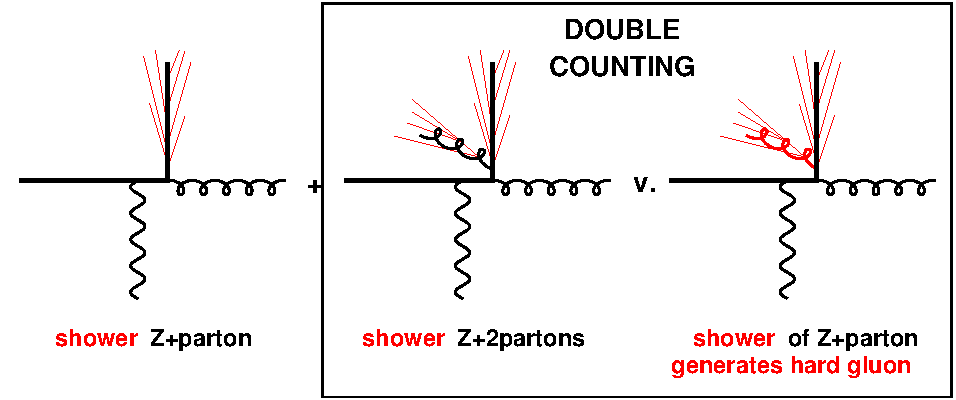
\includegraphics[width=0.8\textwidth]{figures/eventreco_generation/overlap}
  \caption{ Illustration of the double-counting issues that can arise if one naively attempts to
shower $\cPZ+$parton and $\cPZ+2$parton events. Partons generated by the matrix element are
shown in black, whereas the effects of the parton shower are shown in red. Showering the 1-parton
sample could lead to the generation of a hard gluon, which is already included in the matrix-element
description of the 2-parton sample, leading to a double-counting. Figure taken from
Ref.~\cite{Salam:2010zt}. 
  \label{fig:overlap}}
\end{figure}


For each event generated by \MADGRAPH according to the considered hard process, we want to
find out how it looks from a parton shower point of view. To arrive at this ``equivalent parton
shower history", we cluster the final state partons. The reason this is done, is to obtain
a smooth transition from the matrix element to the parton shower dominated region. 

The clustering is performed using the $k_\text{T}$ jet algorithm, which defines the following two
distance measures,
\begin{align}
  k^2_{\mathrm{T},i\text{beam}} &= p_{\mathrm{T},i}^2 + m_i^2, \\ 
  k^2_{\mathrm{T},ij} &= \Delta R_{ij} \min (p_{\mathrm{T},i}^2 , p_{\mathrm{T},j}^2) + \max (m_i^2,
m_j^2),
\end{align}
with $\Delta R^2_{ij} = 2 (\cosh \Delta y - \cos \Delta\phi)$. The standard $k_\text{T}$ clustering
starts by finding the smallest of the $k^2_{\mathrm{T},ij}$ or $k^2_{\mathrm{T},i\text{beam}}$, and
combining those two partons $i$ and $j$. The combination then replaces the original two partons, and
the clustering is repeated. This continues until there is only a $2 \rightarrow 1$ or $2 \rightarrow
2$ scattering left. 
To obtain the equivalent parton shower history, a few modifications to the standard $k_\text{T}$
clustering are made. 
\begin{itemize}
  \item Only clusterings that correspond to actual Feynman diagrams of the considered model are
included. Two quarks of different flavour will thus never be clustered.  
  \item 
\end{itemize}




% The essential problem that leads to matrix-element/parton-shower matching can be illustrated in a
% very simple way. Assume we have computed the LO cross section for some process, F , and that we
% have added an LL shower to it, as in the left-hand pane of figure 12. We know that this only gives
% us an
% LL description of F + 1. We now wish to improve this from LL to LO by adding the actual LO matrix
% element for F + 1. Since we also want to be able to hadronize these events, etc, we again add an LL
% shower off them. However, since the matrix element for F + 1 is divergent, we must restrict it to
% cover
% only the phase-space region with at least one hard resolved jet, illustrated by the half-shaded
% boxes in
% the middle pane of figure 12. Adding these two samples, however, we end up counting the LL terms
% of the inclusive cross section for F + 1 twice, since we are now getting them once from the shower
% off F and once from the matrix element for F + 1, illustrated by the dark shaded (red) areas of the
% right-hand pane of figure 12. This double-counting problem would grow worse if we attempted to add
% more matrix elements, with more legs. The cause is very simple. Each such calculation corresponds
% to an inclusive cross section, and hence naive addition would give
% σtot = σ0;incl + σ1;incl = σ0;excl + 2 σ1;incl .
% (58)
% Instead, we must match the coefficients calculated by the two parts of the full calculation —
% showers
% and matrix elements — more systematically, for each order in perturbation theory, so that the
% nesting
% of inclusive and exclusive cross sections is respected without overcounting.

% Given a parton shower and a matrix-element generator, there are fundamentally three different
% ways in which we can consider matching the two [34]:
% 1. Slicing: The most commonly encountered matching type is currently based on separating
% (slicing) phase space into two regions, one of which is supposed to be mainly described by hard
% matrix
% elements and the other of which is supposed to be described by the shower. This type of approach
% was first used in H ERWIG [50], to include matrix-element corrections for one emission beyond the
% basic hard process [51, 52]. This is illustrated in figure 13. The method has since been generalized
% by several independent groups to include arbitrary numbers of additional legs [53–57]. Effectively,
% the shower approximation is set to zero above some scale (either due to the presence of explicit
% dead
% zones in the shower, as in H ERWIG, or by vetoing any emissions above a certain matching scale, as
% in
% the (L)-CKKW [53, 54, 56] and MLM [55, 57] approaches), causing the matched result to be identical
% to the matrix element (ME) in that region, modulo higher-order corrections. We may sketch this as
% ME
% corrections
% Matched (above matching scale) = Exact × (1 + O(αs )) ,
% (59)
% where the “shower-corrections” include approximate Sudakov factors and αs reweighting factors ap-
% plied to the matrix elements in order to obtain a smooth transition to the shower-dominated region.
% Below the matching scale, the small difference between the matrix elements and the shower approx-
% imation can be dropped (since their leading singularities are identical and this region by
% definition
% includes no hard jets), yielding the pure shower answer in that region,
% shower
% Matched (below matching scale)
% =
% =
% correction
% Approximate + (Exact − Approximate)
% Approximate + non-singular
% → Approximate .
% This type of strategy is illustrated in figure 14. Since this strategy is discontinuous across phase
% space, a main point here is to ensure that the behaviour across the matching scale be as smooth as
% possible. CKKW showed [53] that it is possible to remove any dependence on the matching scale
% through NLL precision by careful choices of all ingredients in the matching; technical details of
% the
% implementation (affecting the O(αs ) terms in eq. (59)) are important, and the dependence on the
% unphysical matching scale may be larger than NLL unless the implementation matches the theoretical
% algorithm precisely [54, 56, 58]. One should also be aware that all strategies of this type are
% quite
% computing intensive. This is basically due to the fact that a separate phase-space generator is
% required
% for each of the n-parton correction terms, with each such sample a priori consisting of weighted
% events
% such that a separate unweighting step (often with quite low efficiency) is needed before an
% unweighted
% sample can be produced.




\subsection{Hadronization \label{sec:event_hadronization}}

Real events do not consist of partons but of hadrons. Therefore, the set of post-shower partons
must be transformed into a set of primary hadrons, which can then decay further. 
Hadronization is a non-perturbative transition taking place at the hadronization scale. In the
event generation context this scale is by construction identical to the cutoff (resolution) scale of
the parton shower.
Since we have no idea how to calculate the transition between partons and hadrons from first
principles, event generators use QCD-inspired phenomenological models.
Although non-perturbative QCD is not solved, we do have some knowledge of the properties
that such a solution must have. 
An important result from lattice QCD calculations is that the potential of the colour dipole field
between a charge and an anticharge appears to grow linearly with the separation of the charges, when
the separation is greater than about a femtometer. This is known as \textit{linear confinement}, and
is used as a starting point for the string model of hadronization.
The most widely used model is the Lund model, which is implemented in \textsc{Pythia}.

Let us consider the production of a $\cPq\bar{\cPq}$ pair. As the quarks move apart,
linear confinement implies that a potential
\begin{equation}
  V(r) = \kappa r
\end{equation}
is expected at large distances $r$.  This is exactly the potential describing a
string with tension $\kappa$. We can thus interpret this as a colour flux tube that is being
stretched
between the quark and the antiquark. From hadron mass spectroscopy the string tension is
measured to be about $1\GeV/\unit{fm}$.
As the $\cPq$ and $\bar{\cPq}$ move apart, their kinetic energy is gradually converted to potential
energy, stored in the growing string spanned between them. 
Quark-antiquark fluctuations inside the string field can become real particles by absorbing energy
from the string. The original endpoint charges are then screened from each other and the
string breaks into two separate colour-singlet pieces, $(\cPq \bar{\cPq}) \rightarrow (\cPq
\bar{\cPq}') + (\cPq' \bar{\cPq})$. This process continues until only hadrons remain.
Since the string breaks are causally disconnected, they do not have to be considered in any
specific time-ordered sequence. In the Lund model, the string breaks are generated starting
with the hadrons containing the endpoint quarks, and iterating inwards towards the centre of the
string, alternating randomly between the left- and right-hand sides, allowing a single on-shell
hadron to be split off in each step. 

The details of the individual string breaks are not known from first principles. The Lund model
uses the idea of quantum mechanical tunneling, which leads to a flavour-independent
Gaussian spectrum for the transverse momentum (w.r.t. the flux tube) of the $\cPq \bar{\cPq}$ pairs.
Baryon production can be incorporated by allowing string breaks to occur by the production of
pairs of so-called diquarks, loosely bound states of two quarks in a color antitriplet state. 
Because the knowledge of hadronization is incomplete, experimental input is needed to tune many of
the parameters describing the finer details, such as flavor composition, and the ratio of vector to
pseudoscalar mesons. 
